\documentclass[tikz,border=6pt]{standalone}
\usepackage{tikz}
\usetikzlibrary{arrows.meta, decorations.markings, positioning}

\tikzset{
  flow/.style={
    thick, -{Stealth[length=3mm]},
    postaction={decorate},
    decoration={markings, mark=at position 0.55 with {\arrow{Stealth[length=2.5mm]}}}
  },
  fp/.style={circle, draw=black, fill=white, inner sep=1.6pt},
  fpIR/.style={circle, draw=red!70!black, fill=red!70!black, inner sep=2pt},
  fpUV/.style={circle, draw=blue!70!black, fill=blue!70!black, inner sep=2pt},
}

\begin{document}
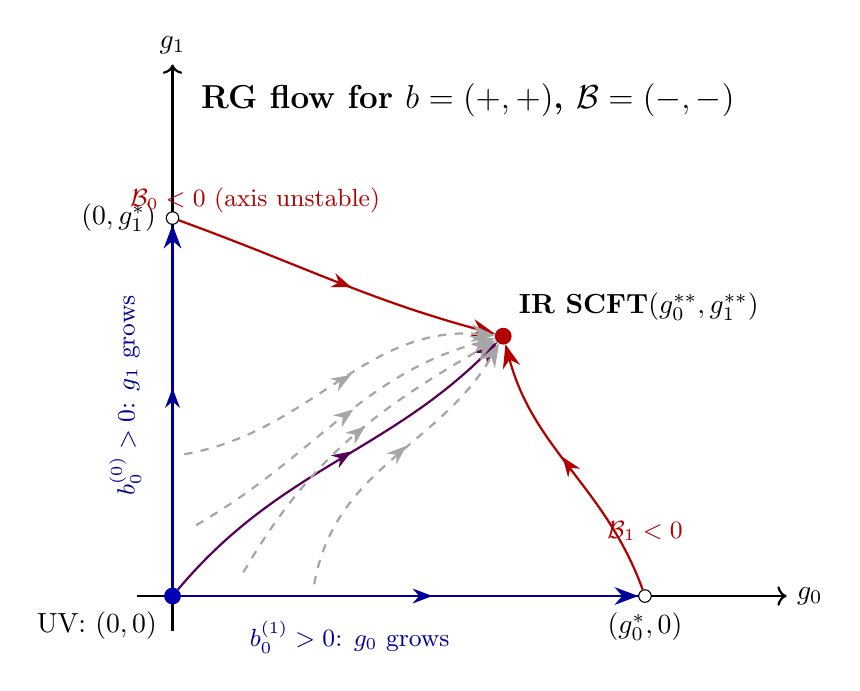
\begin{tikzpicture}[scale=1.5]

  % axes
  \draw[->, thick] (-0.3,0) -- (5.2,0) node[right] {$g_0$};
  \draw[->, thick] (0,-0.3) -- (0,4.5) node[above] {$g_1$};

  % fixed points
  \node[fpUV, label={below left:UV: $(0,0)$}] (UV) at (0,0) {};
  \node[fp,   label={left:$(0, g_1^*)$}]      (A1) at (0,3.2) {};
  \node[fp,   label={below:$(g_0^*, 0)$}]      (A0) at (4.0,0) {};
  \node[fpIR, label={above right:\textbf{IR SCFT}\\$(g_0^{**}, g_1^{**})$}, align=left]
        (IR) at (2.8,2.2) {};

  % on-axis flows: UV -> axis SCFTs (b_0>0 so couplings grow)
  \draw[flow, blue!60!black] (UV) -- (A1);
  \draw[flow, blue!60!black] (UV) -- (A0);

  % off-axis repulsion from axis SCFTs (B_a < 0)
  \draw[flow, red!70!black] (A1) to[out=-20, in=165] (IR);
  \draw[flow, red!70!black] (A0) to[out=110, in=-75] (IR);

  % interior flow from UV directly to IR
  \draw[flow, violet!70!black] (UV) to[out=50, in=225] (IR);

  % a couple of generic trajectories
  \draw[flow, gray!70, dashed] (0.6,0.2) to[out=60, in=210] (IR);
  \draw[flow, gray!70, dashed] (0.2,0.6) to[out=30, in=195] (IR);
  \draw[flow, gray!70, dashed] (1.2,0.1) to[out=80, in=240] (IR);
  \draw[flow, gray!70, dashed] (0.1,1.2) to[out=10, in=175] (IR);

  % sign labels
  \node[red!70!black]  at (0.7, 3.35) {\small $\mathcal{B}_0 < 0$ (axis unstable)};
  \node[red!70!black]  at (4.0, 0.55) {\small $\mathcal{B}_1 < 0$};
  \node[blue!60!black] at (1.5, -0.35) {\small $b_0^{(1)}>0$: $g_0$ grows};
  \node[blue!60!black, rotate=90] at (-0.4, 1.7) {\small $b_0^{(0)}>0$: $g_1$ grows};

  % title
  \node at (2.5, 4.2) {\large\bfseries RG flow for $b=(+,+)$, $\mathcal{B}=(-,-)$};

\end{tikzpicture}
\end{document}
